

\subsection{Cross Sections as a function of the Transverse Momentum Imbalance perpendicular to the Muon Transverse Momentum }

The differential cross section as a function of \tkidptx \ for interactions on the CH, C, H$_{2}$O, Fe, and Pb targets, respectively, are shown in Fig.~\ref{figure:xsec_dptx}. This variable is the component of \tkidelta \ that is perpendicular to the muon direction.  The width is sensitive to nuclear effects and it should be symmetric around zero.  The uncertainties broken down by source for both the absolute cross sections and the cross section ratios as a function of \tkidptx\ can be found in Fig.~\ref{fig:xsec_err_dptx}.

% tki_dptx xsecs
\begin{figure}[h]  
	\centering
  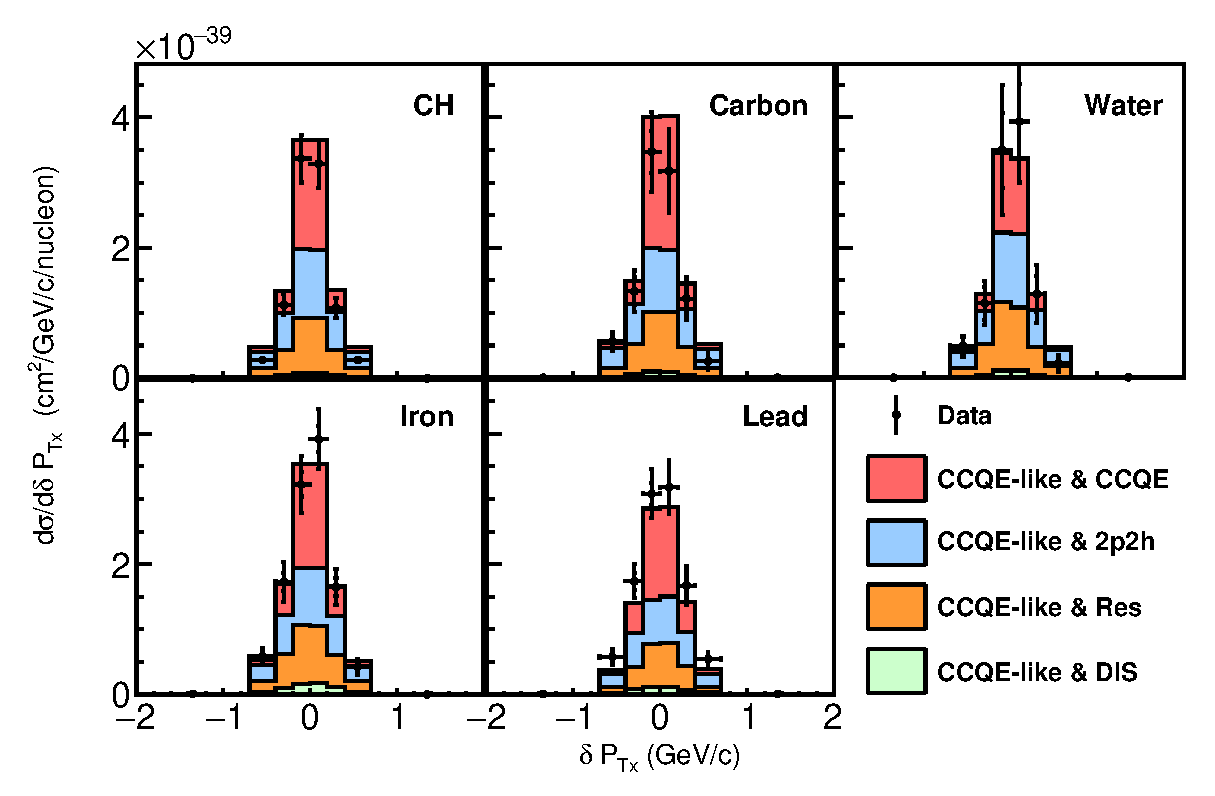
\includegraphics[width=\linewidth]{Figures/xsec_five_square/dptx.eps}
	\caption{The differential cross section as a function of \tkidptx \ for CH, C, H$_{2}$O, Fe, and Pb targets, along with the predictions for the different quasielastic-like signal processes.}
	\label{figure:xsec_dptx}
\end{figure}

These results show no evidence of the left-right  asymmetry in \tkidptx \ for interactions on scintillator that was observed earlier with marginal significance in the LE data~\cite{MINERvA:2019ope}. Also, the asymmetry is not in evidence in the data taken on any of the other nuclear targets.  Improvements in the background tuning and subtraction procedure allowing for asymmetric backgrounds is thought to be the probable reason behind this change.

The width of the QE part of this variable is expected to arise from Fermi smearing.  FSI and 2p2h and resonant processes give broader contributions to the width of this variable.  Note that the data is somewhat narrower than the MINERvA tune expectation for interactions on scintillator and carbon.  This is similar to what was seen in the LE data~\cite{MINERvA:2019ope}.  For the interactions on Pb, the data is broader than the simulation.

The differential cross section as a function of \tkidptx \ for the different targets as compared to a range of models is given in Fig.~\ref{fig:models_dptx}. Again the data are covered by the range of models.  NEUT and the hN versions of GENIE tend to overpredict the cross section as compared to the data, particularly for the larger targets. The other models do a fairly good job describing the data.  The \chisq\ between the cross sections and the models can be found in Table~\ref{tab:dptx}.

% comparisons to generators dptx
\begin{figure}
    \centering
        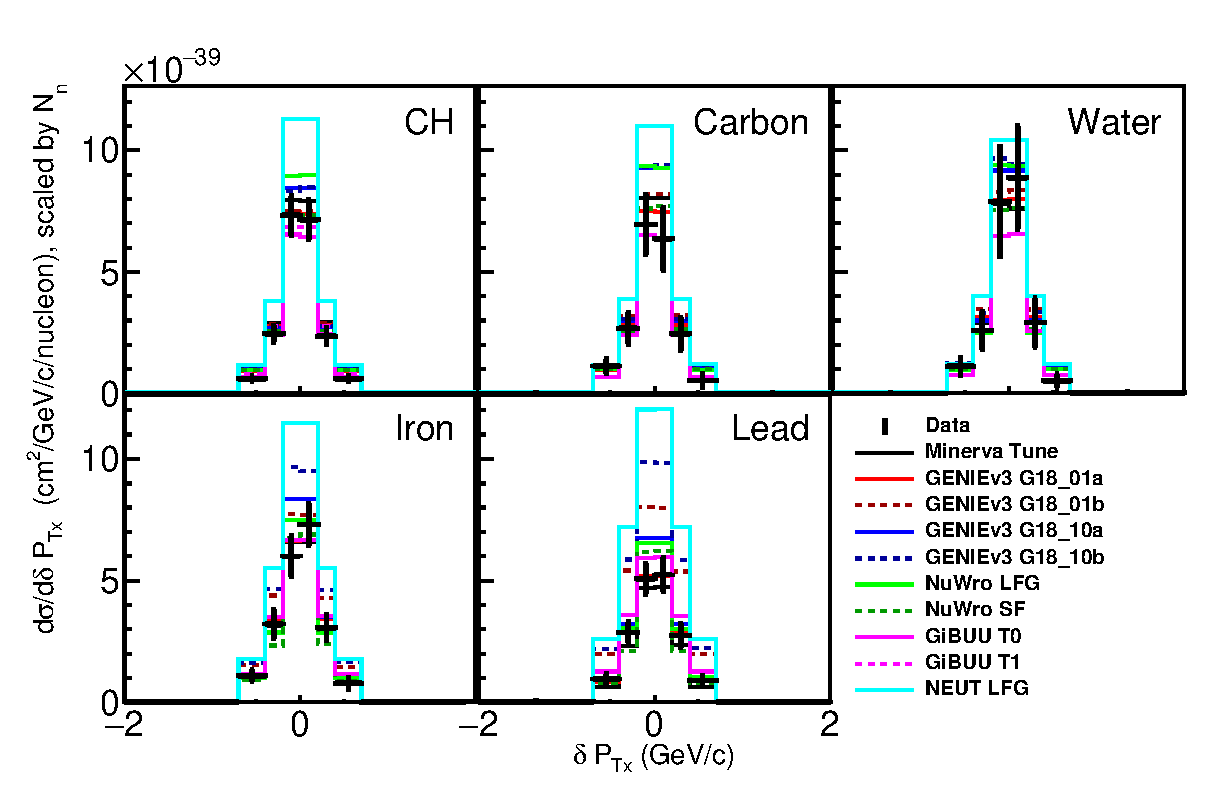
\includegraphics[width=\linewidth]
         {Figures/gencompare/dptx_5square.eps}
    \caption{Cross section measurements and predictions as a function of \tkidptx\ for different targets and for a selection of different generator and model choices.}
    \label{fig:models_dptx}
\end{figure}

The ratio of the differential cross section as a function of  \tkidptx \ for each nuclear target (C, H$_{2}$O, Fe, Pb) to that for scintillator is shown in 
Fig.~\ref{Fig:ratios_dptx}. The models reproduce the data fairly well in these ratios except in the tails of Fe and Pb where the FSI is expected to play a large role.  
The \chisq\ between the cross section ratios and the models can be found in Table~\ref{tab:dptx}.

\begin{figure}
    \centering
        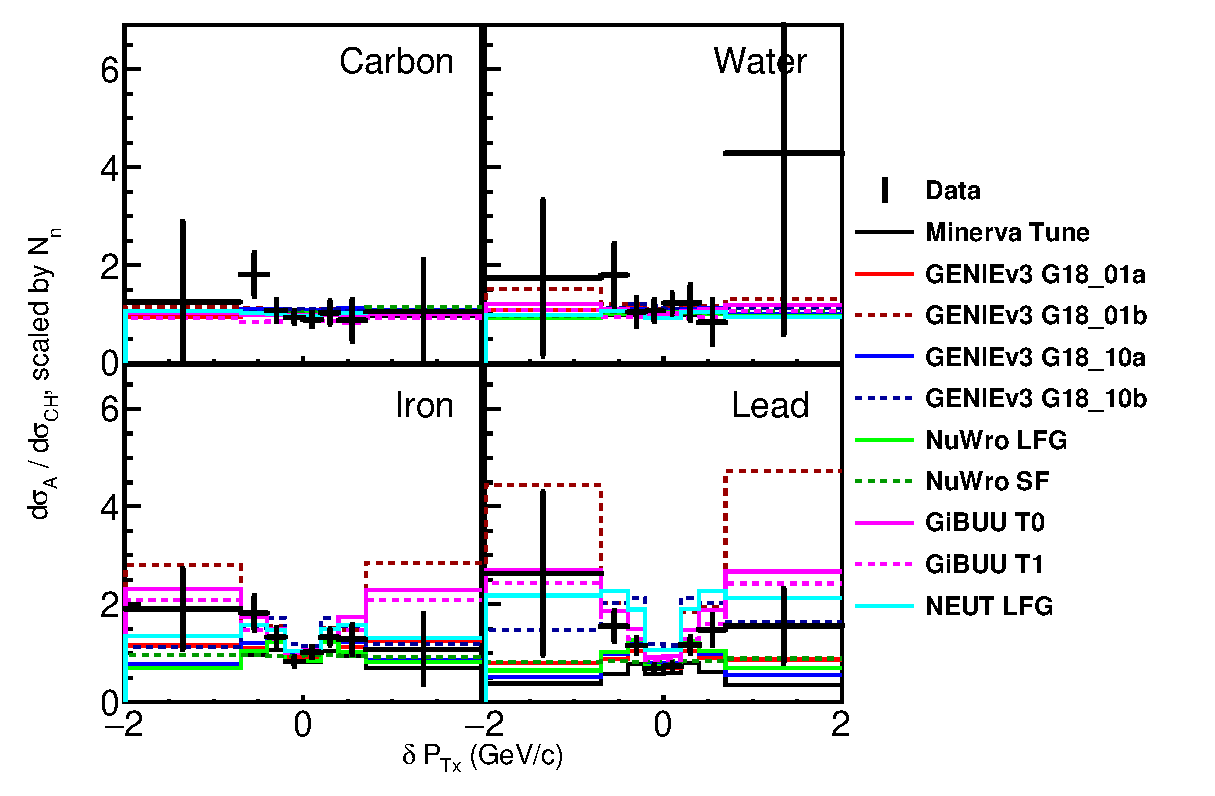
\includegraphics[width=\linewidth]{Figures/gencompare/dptx_4square.eps}
    \caption{\tkidptx\ cross-section ratio comparison for multiple targets.  Note that changes to the FSI model (GENIE ``a'' to ``b'')
     in GENIE change the cross section ratio at extreme positive and negative values of \tkidptx\ more than changes to the 2p2h model (GiBUU T0 to GiBUU T1) or changes to the initial state (GENIE 1 to GENIE 10) or (NuWro LFG to NuWro SF).}
        \label{Fig:ratios_dptx}
\end{figure}